% 使用 xelatex -> biber -> xelatex -> xelatex 编译
\documentclass{hbutthesis}
\addbibresource{references.bib}

\setlength{\headheight}{13pt}

\begin{document}

\setlength{\headheight}{13pt}

\begin{titlepage}
    \vspace*{5mm} 
    {\centering
      \begin{tabularx}{16cm}{@{}R{4.5cm}L{11.5cm}@{}}
        \heiti\zihao{-4}中图分类号:\underline{\makebox[2.25cm][l]{}} &
        \hspace{6.75cm} \heiti\zihao{-4}密\hspace{2em}级:\underline{\makebox[2.25cm][l]{}} \\
        \zihao{-4}{\bfseries U\hspace{0.5em}D\hspace{0.5em}C}\zihao{-4}:\underline{\makebox[2.25cm][l]{}} &
        \hspace{6.75cm} \heiti\zihao{-4}学校代码:\underline{\makebox[2.25cm][l]{\quad 10512}} \\
      \end{tabularx}\par}
    \vspace{1cm}

    {\centering
      
\includegraphics[width=5.9cm,height=1.4cm]{photo/HuBeiUniversity}\par}
    \vspace{-6.5mm}

    {\centering
      \heiti\zihao{0} 硕\hspace{0.3em}士\hspace{0.3em}学\hspace{0.3em}位\hspace{0.3em}论\hspace{0.3em}文
      \vspace{2.05cm}

      %\heiti\zihao{2} 论文题目：\underline{\hbox to 12cm{}} \\[1pt]
      %\underline{\hbox to 16cm{}}\par
      \heiti\zihao{2} 论文题目：\underline{\hbox to 12cm{如何在湖北大学顺利毕业\hfil}} \\[3pt]
      \underline{\hbox to 16cm{  \hfil}}\par
    }
    \vspace{52pt}

    {\centering\renewcommand{\arraystretch}{1.9}
      \begin{tabularx}{\textwidth}{L{2.5cm}@{}L{13.5cm}}
        \heiti\zihao{-3} 研\hspace{0.5em}究\hspace{0.5em}生： & \underline{\makebox[13.25cm][l]{\heiti\zihao{-3} XXX}} \\
        \heiti\zihao{-3} 学\hspace{2em}号： & \underline{\makebox[13.25cm][l]{\heiti\zihao{-3} 20XXXXXXXXXXXXXX}} \\
        \heiti\zihao{-3} 导\hspace{2em}师： & \underline{\makebox[13.25cm][l]{\heiti\zihao{-3} XXX教授、XXX副研究员}} \\
        \heiti\zihao{-3} 专\hspace{2em}业： & \underline{\makebox[13.25cm][l]{\heiti\zihao{-3} XXX}} \\
        \heiti\zihao{-3} 研究方向： & \underline{\makebox[13.25cm][l]{\heiti\zihao{-3} XXX}} \\
      \end{tabularx}\par}

    \vspace{4.55cm}  
    {\centering\textbf{\bfheiti\zihao{-3} 年\hspace{1.5em}月} \par}
\end{titlepage} % 封面
\setlength{\headheight}{13pt}

{\centering
\begin{tabularx}{16cm}{@{}L{8cm}L{8cm}@{}}
  \textbf{\bfheiti\zihao{4}中图分类号}: &
  \hspace{3.25cm} \textbf{\bfheiti\zihao{4}学校代码:10512} \\[5pt]
  \textbf{\bfheiti\zihao{4}学\hspace{1em}号: 20XXXXXXXXXXXXX} &  \\
\end{tabularx}\par}

\vspace{2.5cm}
\begin{center}
  \heiti\zihao{-2}湖北大学硕士学位论文
\end{center}
\vspace{1.5cm}
\begin{center}
  \textbf{\bfheiti\zihao{-1} 如何在湖北大学顺利毕业}
\end{center}
\vspace{4.5cm}

{\centering
  \songti\zihao{4}\renewcommand{\arraystretch}{1.5}
  \begin{tabularx}{16cm}{@{}L{8cm}L{8cm}@{}}
  作者姓名：XXX & \songti\zihao{4}指导教师姓名、职称：XX（教授）\\
  申请学位类别：学术型硕士学位 & 学科专业名称：XXXX \\
  研究方向：XXXXX &  \\
  论文提交日期：\hspace{2em}年\hspace{1.5em}月\hspace{1.5em}日 & 论文答辩日期：\hspace{2em}年\hspace{1.5em}月\hspace{1.5em}日 \\
  学位授予单位：湖北大学  & 学位授予日期：\hspace{2em}年\hspace{1.5em}月\hspace{1.5em}日 \\
  答辩委员会主席：\underline{\makebox[6.5em][l]{}} &  \\             
  \end{tabularx}\par
}
\thispagestyle{empty}

\newpage
\thispagestyle{empty}
{\renewcommand{\arraystretch}{1.5}
\vspace{2cm}
\begin{center}
{\zihao{-2}\bfseries How to Successfully Graduate from Hubei University} \\
\vspace{2.5cm}
{\zihao{4} A Thesis Submitted for the Degree of Master} \\
\vspace{5cm}
{\bfseries\zihao{-3}Candidate：\bfseries\songti XXX \\[15pt]
Supervisor：Prof. XXX XXX, Assoc. Res. XXX XXX} \\
\vfill
{\zihao{-3}
Hubei University \\[15pt] 
Wuhan, China}
\end{center}}

\newpage
\thispagestyle{empty}

\vspace{5mm}
\begin{spacing}{1.5}
{\centering\textbf{\bfheiti\zihao{-2} 学位论文原创性声明}\par}
\vspace{0.9em}
{\songti\fontsize{13pt}{14pt}\selectfont
本人郑重声明：所呈交的论文是本人在导师的指导下独立进行研究所取得的研究成果。除
了文中特别加以标注引用的内容外，本论文不包含任何其他个人或集体已经发表或撰写的
成果作品。对本文的研究做出重要贡献的个人和集体，均已在文中以明确方式标明。本人
完全意识到本声明的法律后果由本人承担。\par
\vspace{1cm}
作者签名：\hspace{6em} 日期：\hspace{2em} 年 \hspace{1.5em} 月 \hspace{1.5em} 日\par
}
\vspace{2cm}
{\centering\textbf{\bfheiti\zihao{-2} 学位论文使用授权书}\par}
\vspace{0.9em}
{\songti\fontsize{13pt}{14pt}\selectfont
本论文作者完全了解学校关于保存、使用学位论文的管理办法及规定，即学校有权保留并
向国家有关部门或机构送交论文的复印件和电子版，允许论文被查阅和借阅，本人授权湖
北大学将本论文的全部或部分内容编入学校认可的有关数据库进行检索，允许论文被汇编
、复制、查阅和进行信息网络传播服务，同时本人保留在其他媒体发表论文的权力。\par
}
%\bigskip
\songti\zihao{-4}
\begin{center}
  \begin{tabularx}{14cm}{@{}L{7cm}L{7cm}@{}}
    学位论文作者签名： & 导师签名： \\
    \vspace{0.9em} & \vspace{0.9em} \\
    \fangsong\zihao{5} \hspace{3em}年 \hspace{2em} 月 \hspace{2em} 日 & \fangsong\zihao{5} \hspace{3em}年 \hspace{2em} 月 \hspace{2em} 日 \\
  \end{tabularx}%
\end{center}
\end{spacing}
	
\thispagestyle{empty} % 声明

\newpage % 新的一页
\thispagestyle{romanfancy}
\pagenumbering{Roman} % 大写罗马数字页码
\begin{center}
  \begin{singlespace}
    \heiti\zihao{2}如何在湖北大学顺利毕业
  \end{singlespace}
\end{center}

\chapter*{摘\hspace{1em}要}
\addcontentsline{toc}{chapter}{摘要}
\vspace{12pt} % 空一行

你的摘要
\vspace{12pt}

\heiti\zihao{-4}【关键词】:\songti latex；模板

\newpage
\thispagestyle{romanfancy}
\begin{center}
  \begin{singlespace}
    \zihao{2}\textbf{How to Successfully Graduate from Hubei University}
  \end{singlespace}
\end{center}

\chapter*{\textbf{Abstract}}
\addcontentsline{toc}{chapter}{Abstract}
\vspace{12pt}

Your abstract
\vspace{12pt}

\heiti\zihao{-4}\textbf{【Keywords】:} \textit{latex}, template

{
  \newpage
  \pagestyle{romanfancy}   % 整个目录都使用该页眉
  \begin{center}
    \tableofcontents      % 章节目录
  \end{center}

  \newpage
  \begin{center}
    \listoffigures        % 图目录
  \end{center}

  \newpage
  \begin{center}
    \listoftables         % 表目录
  \end{center}
}

\pagestyle{fancy}
\newpage
\pagenumbering{arabic} % 阿拉伯数字页码
\setcounter{page}{1} % 设置页码
\chapter{前\hspace{1em}言}

\songti
一定顺利毕业一定顺利毕业一定顺利毕业一定顺利毕业一定顺利毕业一定顺利毕业一定顺利
毕业一定顺利毕业一定顺利毕业一定顺利毕业一定顺利毕业一定顺利毕业一定顺利毕业一定
顺利毕业一定顺利毕业一定顺利毕业一定顺利毕业一定顺利毕业一定顺利毕业。

% 下一段
正文正文正文正文正文正文正文正文正文正文正文正文正文正文正文正文正文正文正文正文
正文正文正文正文正文正文正文正文正文正文正文正文正文正文正文正文正文正文正文正文
正文正文正文正文正文正文正文正文正文正文正文正文正文正文正文正文正文正文正文。

\section{二级标题}

正文正文正文正文正文正文正文正文正文正文正文正文正文正文正文正文正文正文正文正文
正文正文正文正文正文正文正文正文正文正文正文正文正文正文正文正文正文正文正文正文
正文正文正文正文正文正文正文正文正文正文正文正文正文正文正文正文正文正文正文。

正文正文正文正文正文正文正文正文正文正文正文正文正文正文正文正文正文正文正文正文
正文正文正文正文正文正文正文正文正文正文正文正文正文正文正文正文正文正文正文正文
正文正文正文正文正文正文正文正文正文正文正文正文正文正文正文正文正文正文正文。

\subsection{三级标题}

正文正文正文正文正文正文正文正文正文正文正文正文正文正文正文正文正文正文正文正文
正文正文正文正文正文正文正文正文正文正文正文正文正文正文正文正文正文正文正文正文
正文正文正文正文正文正文正文正文正文正文正文正文正文正文正文正文正文正文正文。

正文正文正文正文正文正文正文正文正文正文正文正文正文正文正文正文正文正文正文正文
正文正文正文正文正文正文正文正文正文正文正文正文正文正文正文正文正文正文正文正文
正文正文正文正文正文正文正文正文正文正文正文正文正文正文正文正文正文正文正文。

\subsection{三级标题}

正文正文正文正文正文正文正文正文正文正文正文正文正文正文正文正文正文正文正文正文
正文正文正文正文正文正文正文正文正文正文正文正文正文正文正文正文正文正文正文正文
正文正文正文正文正文正文正文正文正文正文正文正文正文正文正文正文正文正文正文。

\section{XXXXXXXXXXXXXXXXXXXXXXXX}

正文正文正文正文正文正文正文正文正文正文正文正文正文正文正文正文正文正文正文正文
正文正文正文正文正文正文正文正文正文正文正文正文正文正文正文正文正文正文正文正文
正文正文正文正文正文正文正文正文正文正文正文正文正文正文正文正文正文正文正文。

\subsection{XXXXXXXXX}

文献引用方法：XXXX\cite{Zhang2024}，或XXXXXX\cite{Li2025, Rno2020, Peter2000}
正文正文正文正文正文正文正文正文正文正文正文正文正文正文正文正文正文正文正文正文
正文正文正文正文正文正文正文正文正文正文正文正文正文正文正文正文正文正文正文。

图片引用方法：想吃蛋糕~\ref{cake}。正文正文正文正文正文正文正文正文正文正文正文
正文正文正文正文正文正文正文正文正文正文正文正文正文正文正文正文正文正文正文正文
文正文正文正文正文正文正文正文正文正文正文正文正文正文正文正文正文正文正文正文。

\begin{figure}[htbp]
  \begin{center}
    
\includegraphics[width=0.8\linewidth]{figure/cake}
  \end{center}
  \caption[XXXXXX]{XXXXXX\cite{Zhang2024}。} %目录为[]内的内容，正文中为{}内的内容
  \label{cake} % 用于正文的引用
\end{figure}

\subsection{XXXXXXX}

正文正文正文正文正文正文正文正文正文正文正文正文正文正文正文正文正文正文正文正文
正文正文正文正文正文正文正文正文正文正文正文正文正文正文正文正文正文正文正文正文
正文正文正文正文正文正文正文正文正文正文正文正文正文正文正文正文正文正文正文。

\section{研究方案}

\subsection{研究内容}

正文正文正文正文正文正文正文正文正文正文正文正文正文正文正文正文正文正文正文正文
正文正文正文正文正文正文正文正文正文正文正文正文正文正文正文正文正文正文正文正文
正文正文正文正文正文正文正文正文正文正文正文正文正文正文正文正文正文正文正文。

\subsection{拟解决的主要问题}

正文正文正文正文正文正文正文正文正文正文正文正文正文正文正文正文正文正文正文正文
正文正文正文正文正文正文正文正文正文正文正文正文正文正文正文正文正文正文正文正文
正文正文正文正文正文正文正文正文正文正文正文正文正文正文正文正文正文正文正文。

\subsection{技术路线}

正文正文正文正文正文正文正文正文正文正文正文正文正文正文正文正文正文正文正文正文
正文正文正文正文正文正文正文正文正文正文正文正文正文正文正文正文正文正文正文正文
湖北大学（\ulink{https://www.hubu.edu.cn/}）正文正文正文正文正文正文正文。
流程图如图~\ref{technology}。

\begin{figure}[H]
  \begin{center}
    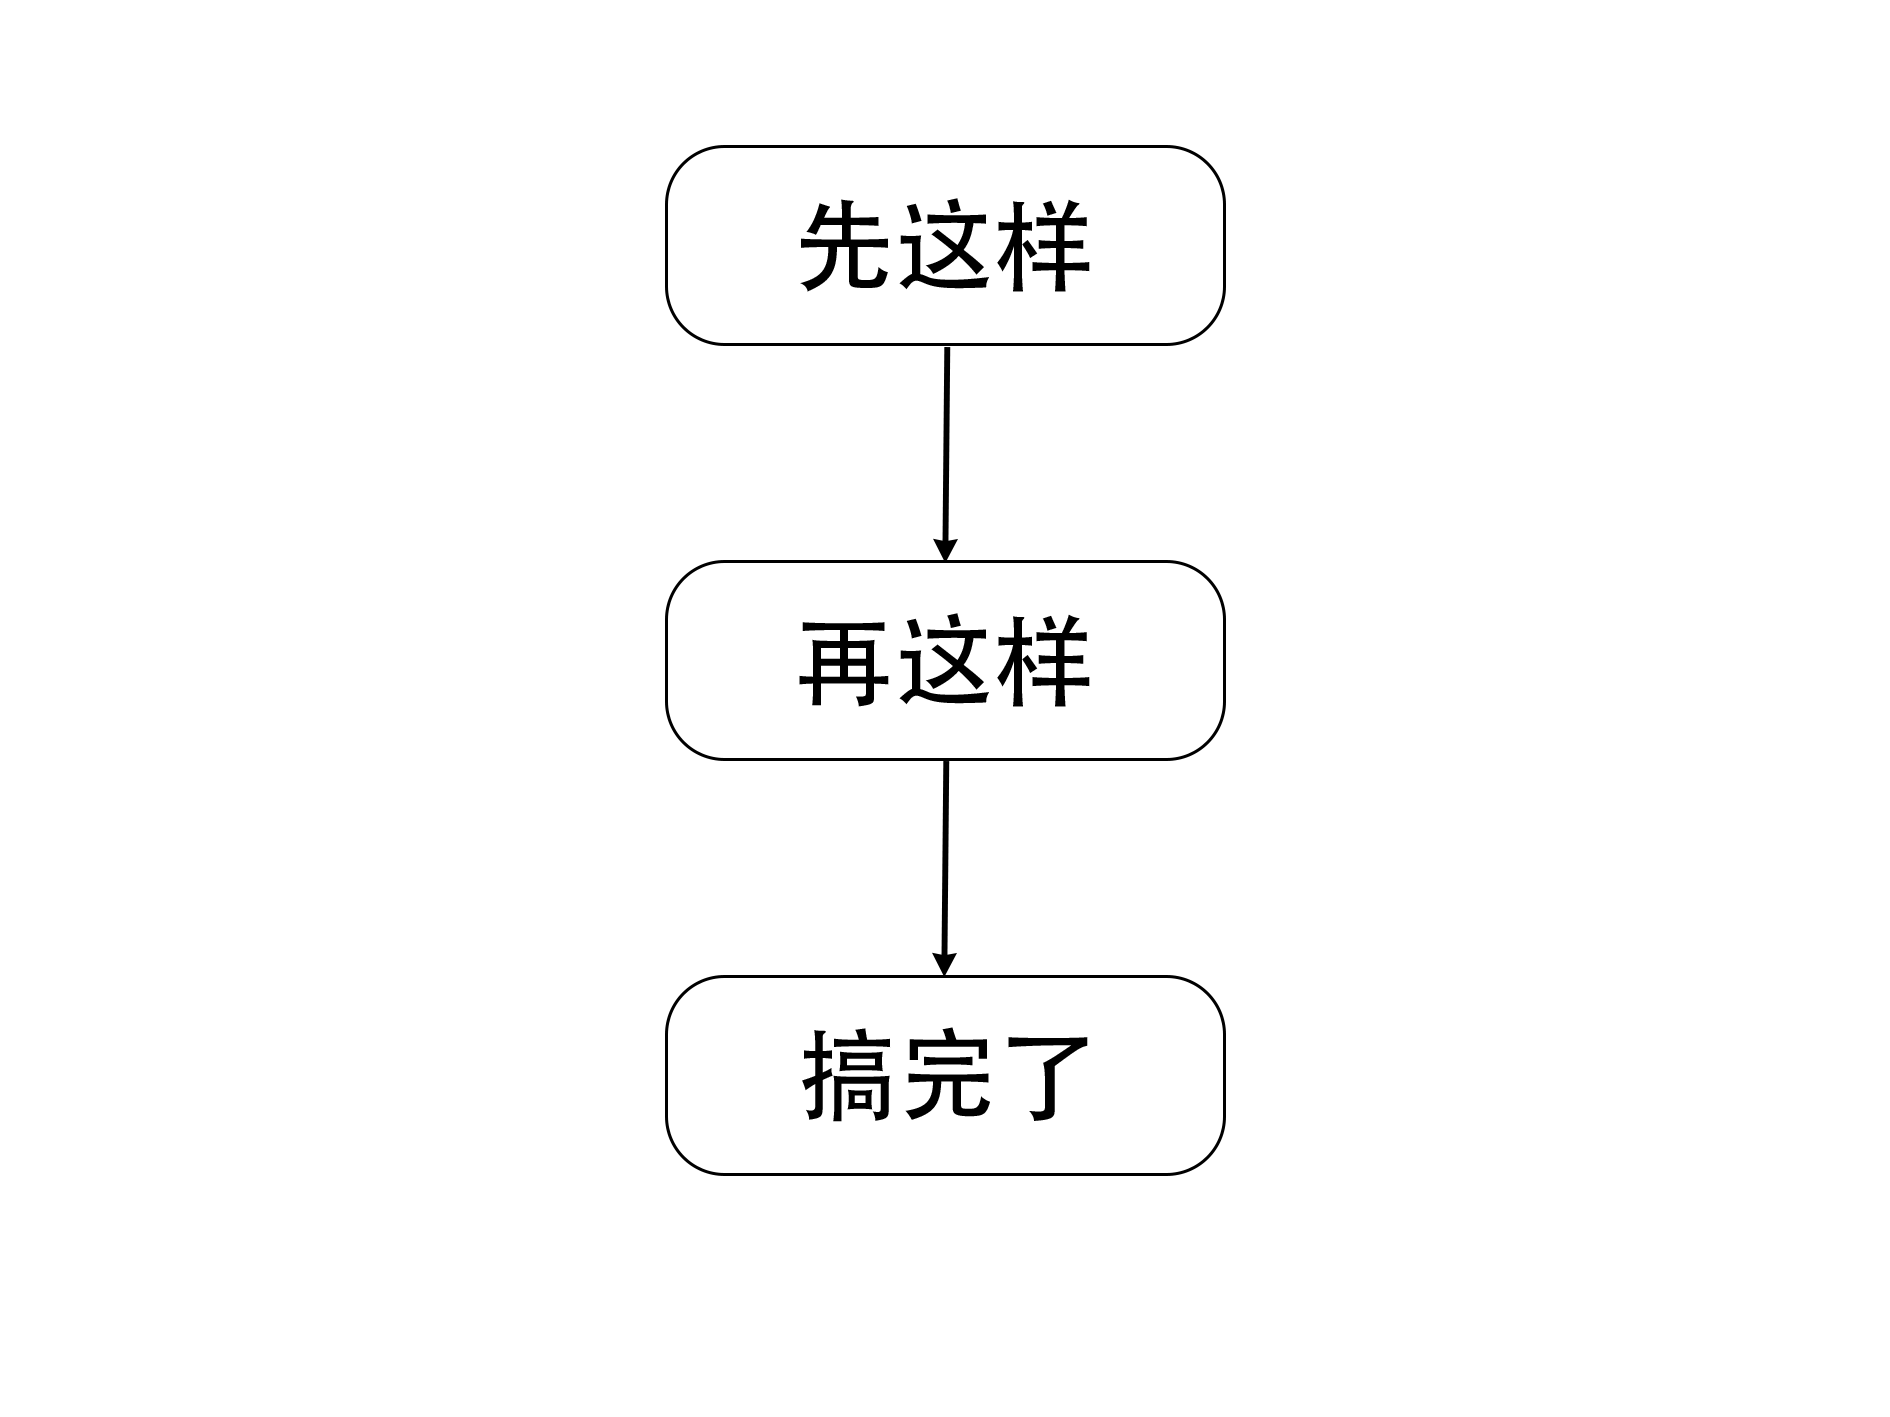
\includegraphics[width=0.9\linewidth]{figure/process}
  \end{center}
  \caption{技术路线流程图}
  \label{technology}
\end{figure}

\newpage
\chapter{材料与方法}

\section{XXXXXXXXX}

正文正文正文正文正文正文正文正文正文正文正文正文正文正文正文正文正文正文正文正文
正文正文正文正文正文正文正文正文正文正文正文正文正文正文正文正文正文正文正文正文
正文正文正文正文正文正文正文正文正文正文正文正文正文正文正文正文正文正文正文。

\section{XXXXXXXXXXX}

正文正文正文正文正文正文正文正文正文正文正文正文正文正文正文正文正文正文正文正文
正文正文正文正文正文正文正文正文正文正文正文正文正文正文正文，计算公式：

\begin{equation}
  \begin{cases}
    \dot{x} = \sigma (y - x) \\ %换行
    \dot{y} = \rho x - y - xz \\
    \dot{z} = xy - \beta z 
  \end{cases}
\end{equation}

式中，$\dot{x}$ 为XXXXXXX，$\dot{y}$ 为XXXXXXXX。其中，XXXXX的 $3 \times 3$ 
XX矩阵为:

\[
\begin{pmatrix}
  a_{11} & a_{12} & a_{13} \\
  a_{21} & a_{22} & a_{23} \\
  a_{31} & a_{32} & a_{33}
\end{pmatrix}
\]

\section{XXXXXXXXXXXXXXXXXX}

正文正文正文正文正文正文正文正文正文正文正文正文正文正文正文正文正文正文正文正文
正文正文正文正文正文正文正文正文正文正文正文正文正文正文正文正，伪代码如下：

\begin{algorithm}[http]
\caption{Calculation of XXXXXX}
\begin{algorithmic}[1] % [1] indicates line numbering
\FOR{each N $i$}
    \STATE $m_i \gets \text{mean(values from X1, X2, X3)}$
    \STATE $T^i = TREE(i)$
\ENDFOR
\STATE Unknown operation
\STATE Unknown operation
\STATE Unknown operation
\end{algorithmic}
\end{algorithm}

\newpage 
\chapter{结果与分析}

\section{图是图我是我}

正文正文正文正文正文正文正文正文正文正文正文正文正文正文正文正文正文正文正文正文
正文正文正文正文正文正文正文正文正文正文正文正文正文正文正文正文正文正文正文正文
正文正文正文正文正文正文正文正文正文正文正文正文正文，如表~\ref{table1}。

正文正文正文正文正文正文正文正文正文正文正文正文正文正文正文正文正文正文正文正文
正文正文正文正文正文正文正文正文正文正文正文正文正文正文正文正文正文正文正文正文
正文正文正文正文正文正文正文正文正文正文正文正文正文，如表~\ref{table2}。

\begin{table}[htbp]
  \centering
  \caption{XXXXXX}
	\label{table1}
  \vspace{-5pt}
  \renewcommand{\arraystretch}{1.5}
  \begin{tabularx}{15cm}{lC{3cm}R{5cm}}
    \toprule
    XX & XXX & XXXXXX \\
    \midrule
    XX & $0 \sim 100$     & XXXX        \\
    XX & $0 \sim 100$     & XXXX        \\
    XX & $0 \sim 100$     & XXXX        \\
    \bottomrule
  \end{tabularx}
\end{table}

\begin{table}[http]
  \centering
  \caption{XXXXXXX}
  \vspace{-5pt}
  \label{table2}
  \renewcommand{\arraystretch}{1.5}
  \begin{tabular}{c | c c c}
    \hline
    \diagbox[dir=NW]{Light on}{Light off} & X &  & Y \\
    \hline
    X   & a & $\Leftarrow$ & b    \\
        & $\Uparrow$  &    &      \\
    Y   & c &              & d    \\
    \hline
  \end{tabular}
\end{table}
% 对于跨页的表格可参考附件 1 的长表格

\section{看看文献的解释套路}

\subsection{XXXXXX}

正文正文正文正文正文正文正文正文正文正文正文正文正文正文正文正文正文正文正文正文
正文正文正文正文正文正文正文正文正文正文正文正文正文正文正文正文正文正文正文正文
正文正文正文正文正文正文正文正文正文正文正文正文正文正文，如图~\ref{lorenz}。

正文正文正文正文正文正文正文正文正文正文正文正文正文正文正文正文正文正文正文正文
正文正文正文正文正文正文正文正文正文正文正文正文正文正文正文正文正文正文正文正文
正文正文正文正文正文正文正文正文正文正文正文正文正文正文正文正文正文正文正文。

\begin{figure}[htbp]
  \begin{center}
    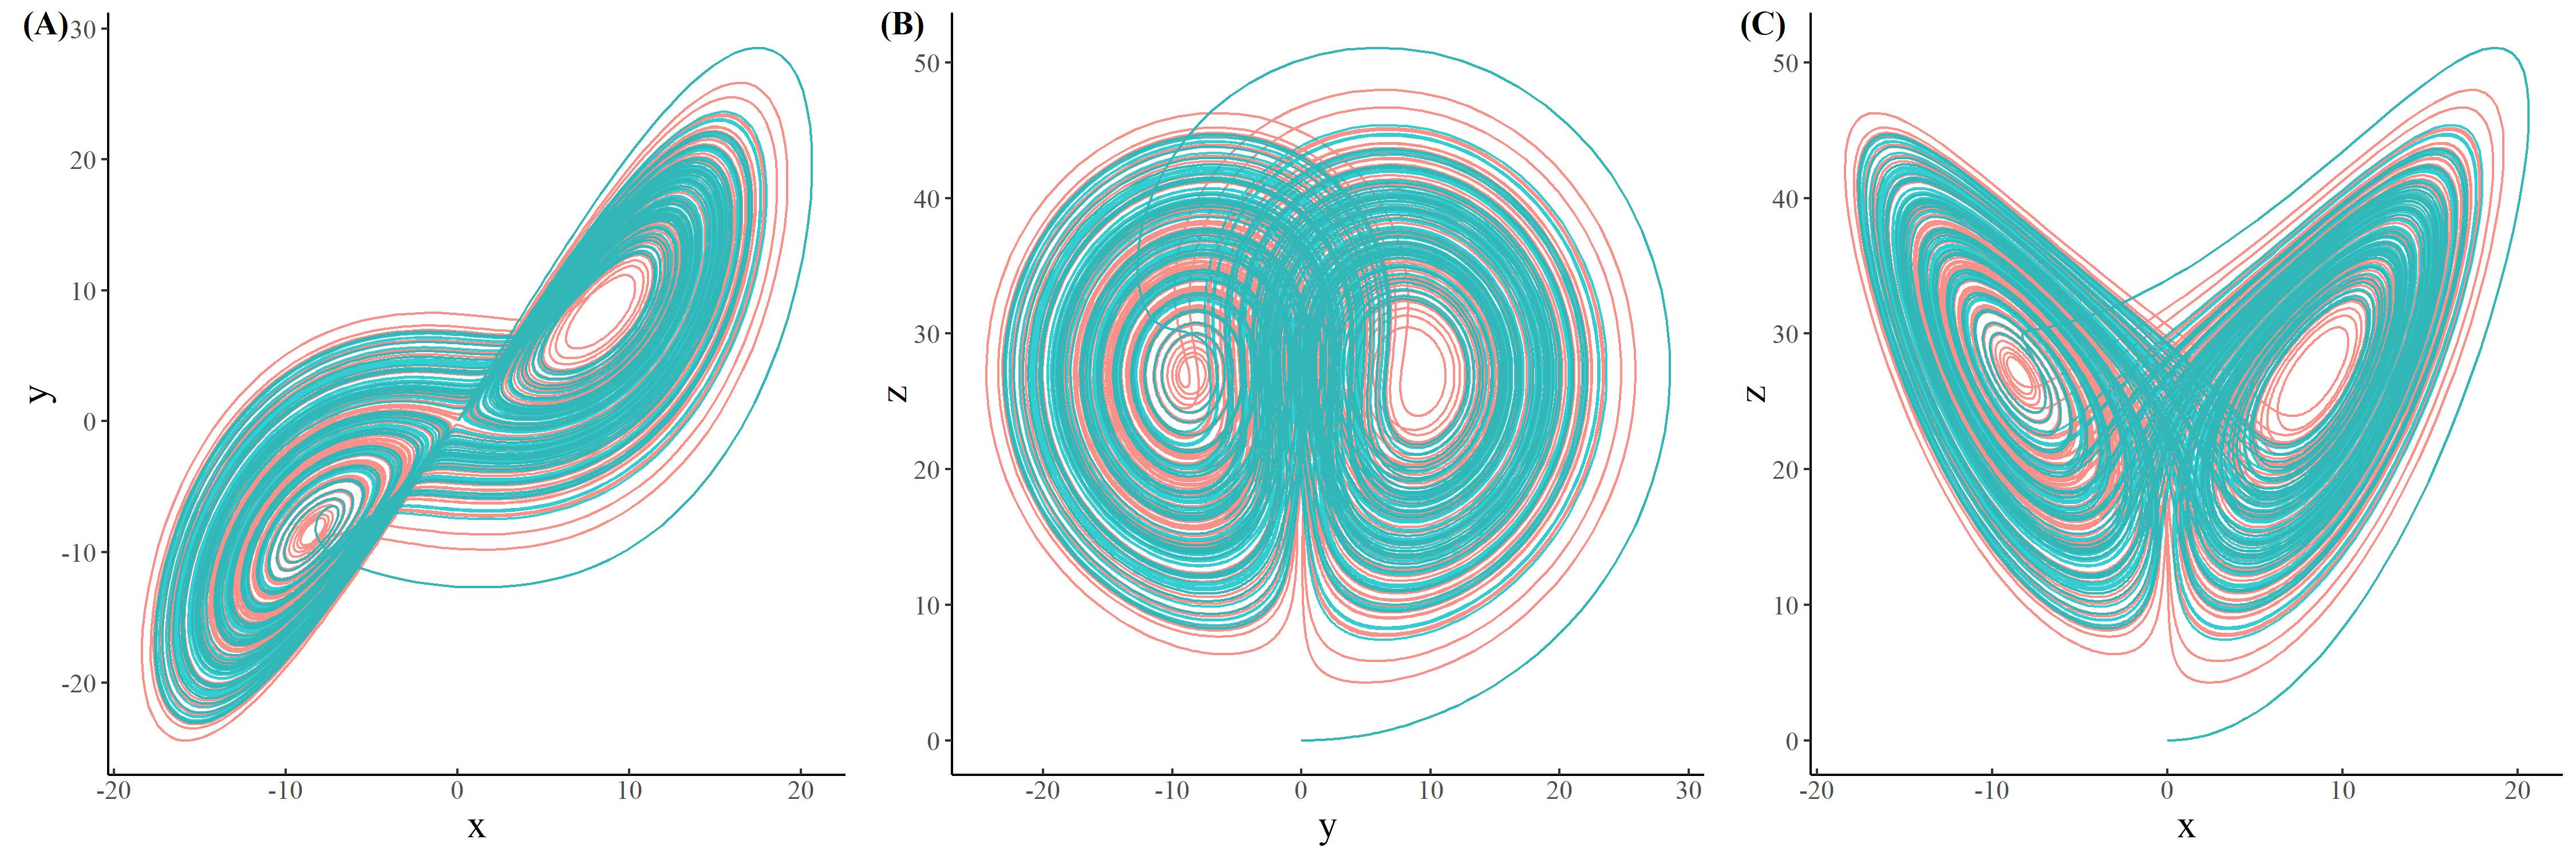
\includegraphics[width=0.95\linewidth]{figure/lorenz.jpeg}
  \end{center}
  \caption{XXXXXX}
  \begin{figcaption}
    (A)\hspace{0.5em}XXXXX。
    (B)\hspace{0.5em}XXXXX。
    (c)\hspace{0.5em}XXXXX。
  \end{figcaption}
  \label{lorenz}
\end{figure}

\subsection{XXXXXX}

正文正文正文正文正文正文正文正文正文正文正文正文正文正文正文正文正文正文正文正文
正文正文正文正文正文正文正文正文正文正文正文正文正文正文正文正文正文正文正文正文
正文正文正文正文正文正文正文正文正文正文正文正文正文正文正文正文正文正文正文。

\section{不会编了}

正文正文正文正文正文正文正文正文正文正文正文正文正文正文正文正文正文正文正文正文
正文正文正文正文正文正文正文正文正文正文正文正文正文正文正文正文正文正文正文正文
正文正文正文正文正文正文正文正文正文正文正文正文正文正文正文正文正文正文正文。

\newpage
\clearpage
\chapter{讨\hspace{1em}论}

\section{改格式}

正文正文正文正文正文正文正文正文正文正文正文正文正文正文正文正文正文正文正文正文
正文正文正文正文正文正文正文正文正文正文正文正文正文正文正文正文正文正文正文正文
正文正文正文正文正文正文正文正文正文正文正文正文正文正文正文正文正文正文正文。

\section{降重}

正文正文正文正文正文正文正文正文正文正文正文正文正文正文正文正文正文正文正文正文
正文正文正文正文正文正文正文正文正文正文正文正文正文正文正文正文正文正文正文正文
正文正文正文正文正文正文正文正文正文正文正文正文正文正文正文正文正文正文正文。

\section{降 AI}

正文正文正文正文正文正文正文正文正文正文正文正文正文正文正文正文正文正文正文正文
正文正文正文正文正文正文正文正文正文正文正文正文正文正文正文正文正文正文正文正文
正文正文正文正文正文正文正文正文正文正文正文正文正文正文正文正文正文正文正文。

\newpage
\markboth{参考文献}{参考文献}
\printbibliography[heading=bibintoc,title={参考文献}] % 请修改 references.bib 文件

\clearpage
\makehbuappendix

\chapter{Supplementary Tables}
%\documentclass{hbutthesis}

\setlength{\headheight}{13pt}

\songti\zihao{5} 

\begin{longtable}{@{\extracolsep{\fill}} l c c l @{}} %长表格
  \caption{XXXXXXX}\label{Appendix1}\\[-5pt]
  \toprule
  xxx &	xxx	& xxx & xxx \\ 
  \midrule
  \endfirsthead 
  \caption{续表} \\[-5pt]
  \toprule
  \endhead
  \bottomrule
  \endfoot 
  \bottomrule
  \endlastfoot 
    xxx & xxx & xxx & xxx \\
    xxx & xxx & xxx & xxx \\
    xxx & xxx & xxx & xxx \\
    xxx & xxx & xxx & xxx \\
    xxx & xxx & xxx & xxx \\
    xxx & xxx & xxx & xxx \\
    xxx & xxx & xxx & xxx \\
    xxx & xxx & xxx & xxx \\
    xxx & xxx & xxx & xxx \\
    xxx & xxx & xxx & xxx \\
    xxx & xxx & xxx & xxx \\
    xxx & xxx & xxx & xxx \\
    xxx & xxx & xxx & xxx \\
    xxx & xxx & xxx & xxx \\
    xxx & xxx & xxx & xxx \\
    xxx & xxx & xxx & xxx \\
    xxx & xxx & xxx & xxx \\
    xxx & xxx & xxx & xxx \\
    xxx & xxx & xxx & xxx \\
    xxx & xxx & xxx & xxx \\
    xxx & xxx & xxx & xxx \\
    xxx & xxx & xxx & xxx \\
    xxx & xxx & xxx & xxx \\
    xxx & xxx & xxx & xxx \\
    xxx & xxx & xxx & xxx \\
    xxx & xxx & xxx & xxx \\
    xxx & xxx & xxx & xxx \\
    xxx & xxx & xxx & xxx \\
    xxx & xxx & xxx & xxx \\
    xxx & xxx & xxx & xxx \\
    xxx & xxx & xxx & xxx \\
    xxx & xxx & xxx & xxx \\
    xxx & xxx & xxx & xxx \\
    xxx & xxx & xxx & xxx \\
    xxx & xxx & xxx & xxx \\
    xxx & xxx & xxx & xxx \\
    xxx & xxx & xxx & xxx \\
    xxx & xxx & xxx & xxx \\
    xxx & xxx & xxx & xxx \\
    xxx & xxx & xxx & xxx \\
    xxx & xxx & xxx & xxx \\
    xxx & xxx & xxx & xxx \\
    xxx & xxx & xxx & xxx \\
    xxx & xxx & xxx & xxx \\
    xxx & xxx & xxx & xxx \\
    xxx & xxx & xxx & xxx \\
    xxx & xxx & xxx & xxx 
\end{longtable}
注：XXXXXX。

\newpage
\chapter{程序代码}
%\documentclass{hbutthesis}

\setlength{\headheight}{13pt}

\songti\zihao{5} 
本研究的 C++ 代码为：

\begin{lstlisting}[language=C++, caption={Fibonacci sequence in C++}]
#include <iostream>
using namespace std;

int fibonacci(int n) {
    if (n <= 1)
        return n;
    return fibonacci(n - 1) + fibonacci(n - 2);
}

int main() {
    int n = 10;
    for (int i = 0; i < n; i++) {
        cout << fibonacci(i) << " ";
    }
    return 0;
}
\end{lstlisting}

本研究的 python 代码为：

\begin{lstlisting}[language=Python, caption={Fibonacci sequence in Python}]
def fibonacci(n):
    if n <= 1:
        return n
    return fibonacci(n - 1) + fibonacci(n - 2)

n = 10
for i in range(n):
    print(fibonacci(i), end=" ")
\end{lstlisting}

本研究的 R 代码为：

\begin{lstlisting}[language=R, caption={Fibonacci sequence in R}]
fibonacci <- function(n) {
  if (n <= 1) {return(n)} else {
    fibonacci(n - 1) + fibonacci(n - 2)
  }
}

10 -> n
for (i in 1 : n) {
  print(fibonacci(i))
}
\end{lstlisting}

\newpage
\thispagestyle{thanks}
\chapter*{致\hspace{1em}谢}
\addcontentsline{toc}{chapter}{致谢}

\setlength{\headheight}{13pt}

\songti
致谢致谢致谢致谢致谢致谢致谢致谢致谢致谢致谢致谢致谢致谢致谢致谢致谢致谢致谢致谢
致谢致谢致谢致谢致谢致谢致谢致谢致谢致谢致谢致谢致谢致谢致谢致谢致谢致谢致谢致谢
致谢致谢致谢致谢致谢致谢致谢致谢致谢致谢致谢致谢致谢致谢致谢致谢致谢致谢致谢。

Ciallo $\sim (\angle~\pmb{\cdot}\,{\scriptstyle \omega}\raisebox{0.2ex}{$\scriptstyle <$}\,)\begin{smallmatrix} \frown \\ \vphantom{a} \end{smallmatrix}$\ding{72}

\end{document}